% =====================================================
% IEEE Conference paper derived from the MAU MSc thesis
% "Spatial Estimation of Air Quality at Unmonitored Locations
%  Using Machine Learning ..." (Abdalazeez Asaad)
% Template: IEEEtran conference (template version 6/27/2024)
% =====================================================
\documentclass[conference]{IEEEtran}
% \IEEEoverridecommandlockouts  % only needed for a funding \thanks; none here

\usepackage{cite}
\usepackage{amsmath,amssymb,amsfonts}
\usepackage{algorithmic}
\usepackage{graphicx}
\usepackage{textcomp}
\usepackage{xcolor}
\usepackage[T1]{fontenc} % added: correct output of Swedish characters a-ring, a-uml, o-uml
\usepackage{booktabs}    % added: result tables
\usepackage{placeins}    % added: \FloatBarrier keeps Fig. 2 from drifting away from RQ3
\graphicspath{{images/}} % added: resolve figures in writing/images/

% added: loosen LaTeX's default reluctance to place a large double-column
% float (figure*) at the top of the page it is cited near, instead of
% deferring it to a separate float page later in the document.
\renewcommand{\dbltopfraction}{0.9}
\renewcommand{\dblfloatpagefraction}{0.85}

\def\BibTeX{{\rm B\kern-.05em{\sc i\kern-.025em b}\kern-.08em
    T\kern-.1667em\lower.7ex\hbox{E}\kern-.125emX}}

\begin{document}

\title{Spatial Estimation of Air Quality at Unmonitored Locations Using
Machine Learning for IoT Sensor Network Design in Swedish Cities}

\author{\IEEEauthorblockN{Abdalazeez Asaad}
\IEEEauthorblockA{\textit{Department of Technology and Society} \\
\textit{Malm\"o University}\\
Malm\"o, Sweden \\
aziz.f1987@gmail.com}
}

\maketitle

\begin{abstract}
Sweden's national air quality reference network produces high-fidelity PM2.5
and NO2 measurements but is spatially sparse, leaving large areas without
direct monitoring. This paper investigates how accurately these pollutants
can be estimated at unmonitored locations, how that accuracy degrades with
distance from the nearest station, and how the resulting relationship can
guide supplementary Internet of Things (IoT) sensor placement. Following a
Design Science Research methodology, a Random Forest model trained on
land-use, topographic, meteorological, and population covariates for 34
reference stations over 2020 to 2024 was evaluated under buffered spatial
leave-one-out cross-validation and benchmarked against inverse distance
weighting (IDW) and land-use regression (LUR). For PM2.5, IDW was the most
accurate estimator, with a mean RMSE of 2.33 against 3.56 micrograms per
cubic metre for Random Forest, indicating that PM2.5 concentrations are
spatially smooth at the national scale. For NO2, Random Forest achieved the
lowest mean RMSE at 7.27 micrograms per cubic metre. Decay curves fitted to
per-station error against distance yielded estimated reliable prediction
distances of approximately 64 km for PM2.5 and 6 km for NO2 under a 50
percent error criterion; both are criterion-dependent estimates. A greedy
sequential placement algorithm applied to the PM2.5 threshold identified 20
candidate sensor locations, raising national land coverage from 10.9 to 67.2
percent and extending coverage to four of Sweden's seven unmonitored regions.
The contribution is a reproducible artefact translating spatial estimation
accuracy into prioritised sensor placement guidance for Swedish municipal air
quality planning.
\end{abstract}

\begin{IEEEkeywords}
air quality, spatial estimation, machine learning, IoT sensor placement,
spatial cross-validation, land-use regression, Sweden
\end{IEEEkeywords}

\section{Introduction}
\label{sec:intro}

Ground-level fine particulate matter (PM$_{2.5}$) and nitrogen dioxide
(NO$_2$) are among the most well-documented contributors to respiratory and
cardiovascular morbidity in European cities, and Swedish urban populations
carry a measurable share of this burden even under a comparatively strict
national regulatory regime \cite{segersson_sweden_health_2017}. Both
pollutants exhibit substantial intra-urban heterogeneity, with concentrations
varying between urban cores, near-road zones, and suburban areas
\cite{sweden_dispersion_2024}, so characterising exposure requires monitoring
at a commensurate spatial resolution.

The Swedish Meteorological and Hydrological Institute (SMHI) operates the
national network of regulatory-grade reference stations. These instruments
meet EU reference methods but are sparse by design, and can be separated by
tens of kilometres; concentrations between them must be estimated rather than
measured. Low-cost Internet of Things (IoT) sensors based on electrochemical
and optical technologies can supplement this network at a fraction of the cost
of a reference station \cite{karinthi_sustainable_aqm_2022, popescu_iot_aq_2024}.
Their placement, however, is typically governed by
property access, power availability, and local intuition rather than by any
analysis of where estimation from the existing network is already adequate and
where a physical sensor is genuinely warranted. A principled placement
criterion requires knowing how estimation accuracy behaves as a function of
distance from the nearest reference station, a relationship that has not been
quantified for the SMHI network.

This paper quantifies that accuracy-distance relationship and uses it to
derive supplementary sensor placement guidance, within a Design Science
Research (DSR) methodology \cite{peffers_dsr_2007,
hevner_design_science_2004}. Three research questions are addressed:

\begin{itemize}
\item \textbf{RQ1:} How accurately can machine learning models estimate daily
PM$_{2.5}$ and NO$_2$ at spatially withheld SMHI reference stations using
land-use, topographic, and meteorological covariates?
\item \textbf{RQ2:} How does estimation accuracy degrade with distance from the
nearest active reference station, and what is the reliable prediction distance
threshold?
\item \textbf{RQ3:} How can optimisation heuristics guide the placement of IoT
sensor nodes across Sweden, prioritising regions where estimation uncertainty
is highest?
\end{itemize}

The contributions are: (i) an evaluation of spatial PM$_{2.5}$ and NO$_2$
estimation for Sweden under a buffered spatial leave-one-out protocol that
suppresses near-neighbour leakage; (ii) parametric decay curves relating
estimation error to distance from the nearest station, and criterion-dependent
reliable prediction distances of approximately 64~km (PM$_{2.5}$) and 6~km
(NO$_2$); (iii) a greedy sequential placement artefact that translates the
PM$_{2.5}$ threshold into 20 prioritised national sensor locations; and (iv)
evidence that a deployment sized for one pollutant's spatial behaviour does not
serve the other.

\section{Related Work}
\label{sec:related}

\textit{Regulatory monitoring and its limits.} Air quality monitoring in
Europe operates through a hierarchy of infrastructure, with regulatory
reference stations at the top producing measurements that conform to EU
reference methods and form the basis for national reporting. In Sweden this
function is fulfilled by the SMHI network. Segersson et al.
\cite{segersson_sweden_health_2017} attribute substantial cardiovascular and
respiratory mortality in Stockholm, Gothenburg, and Ume\r{a} to traffic-related
PM$_{2.5}$ and NO$_2$ at concentrations that may remain below EU limit values,
and high-resolution dispersion modelling confirms that intra-urban exposure
gradients in contemporary Swedish cities are large
\cite{sweden_dispersion_2024}. Reference stations are sited to represent broad
background zones rather than local conditions, so the areas between them have
no direct measurement record. Munera et al.
\cite{munera_iot_aq_smart_cities_2021} find in a systematic mapping study that
monitoring capability in IoT air quality projects often outpaces its use in
actual planning.

\textit{Spatial estimation methods.} Inverse distance weighting (IDW)
estimates a concentration as a distance-weighted average of nearby
observations and makes no assumption about the drivers of spatial variation,
but remains a standard deterministic baseline. Land-use regression (LUR) is
the established peer-reviewed standard for long-run outdoor concentrations in
Europe: Hoek et al. \cite{hoek_lur_review_2008} review 25 studies, and the
European Study of Cohorts for Air Pollution Effects (ESCAPE) reports a
cross-validation coefficient of determination (R$^2$) of about 0.71 for
PM$_{2.5}$ \cite{eeftens_escape_pm_2012} and a leave-one-out R$^2$ of 0.83 for
NO$_2$ \cite{wang_escape_no2_2013}. Machine learning methods are increasingly
applied for their capacity to model non-linear predictor interactions, with
reviews reporting consistent root mean squared error (RMSE) and mean absolute
error (MAE) improvements over regression baselines
\cite{agbehadji_ml_aq_review_2024, chen_pm25_interpolation_2021}.

\textit{Validation and placement optimisation.} When training data are
spatially autocorrelated, standard random cross-validation underestimates
prediction error, because nearby stations share similar predictor environments
and concentrations; block-based or location-withholding strategies are
recommended instead \cite{roberts_spatial_cv_2017, valavi_blockcv_2019}. Given
a model of estimation uncertainty, sensor placement can be framed as an
optimisation problem. Particle Swarm Optimization has been applied to outdoor
placement within a single monitoring area \cite{gupta_pso_placement_2023, pso_node_deployment_2024},
but placement grounded in an empirically derived
model of estimation error as a function of distance from an existing national
network remains largely unexplored.

Three gaps follow. First, the accuracy achievable at genuinely unmonitored
Swedish locations under a spatial validation protocol is not established.
Second, the distance-accuracy relationship for the SMHI network has not been
quantified. Third, national-scale IoT placement anchored in such a
relationship has not been demonstrated for Sweden. RQ1 to RQ3 address these in
turn.

\section{Methodology}
\label{sec:method}

The study follows the six-phase DSR process of Peffers et al.
\cite{peffers_dsr_2007}: the sparse SMHI network and the absence of a
placement criterion define the problem; RQ1 to RQ3 define the solution
objectives; the estimation model, decay analysis, and placement algorithm
below constitute design and development; and the artefact is demonstrated on
Sweden nationally and evaluated by coverage gain, following the design-science
rigour guidelines of Hevner et al. \cite{hevner_design_science_2004}.

\subsection{Data}
\label{sec:method-data}

Five open datasets are combined. Daily mean PM$_{2.5}$ and NO$_2$ for 1
January 2020 to 31 December 2024 were obtained from SMHI for 34 reference
stations. A completeness filter of 90 percent of daily records per station and
pollutant is applied; 11 stations pass concurrently for both pollutants and
form the spatially independent validation sample, while all 34 may contribute
training rows. Meteorological covariates (temperature, wind, humidity,
precipitation) come from the nearest SMHI surface station per parameter; land
use from CORINE Land Cover 2018 and topography from EU-DEM v1.1, both 100~m
rasters; and population from the JRC GEOSTAT 2018 1~km grid. All layers are
projected to ETRS89 LAEA (EPSG:3035). The joined daily feature matrix has
48{,}283 rows.

\subsection{Feature Set}

Thirty predictors span six groups: 18 CORINE land-use proportions (nine
functional classes at 500~m and 1~km buffers), two topographic (elevation and
terrain roughness within 1~km), two population (counts within 1~km and 5~km),
five meteorological (wind speed, wind direction, temperature, relative
humidity, precipitation), two positional (latitude, longitude), and one binary
indicator for the 2020--2021 COVID-19 period. No explicit feature selection is
applied; with only 11 spatially independent units, the bootstrap aggregation
of Random Forest acts as implicit regularisation.

\subsection{Estimators}

Three estimators are fitted independently within each validation fold.
\textit{IDW} is the deterministic baseline, weighting observed stations by
$1/d^{2}$. \textit{LUR} is ordinary least squares on the 30 features,
representing the established European benchmark \cite{hoek_lur_review_2008}.
\textit{Random Forest} (RF) is the primary model: 200 trees, a minimum of five
samples per leaf, and a fixed seed. RF is selected for its documented accuracy
over LUR across data environments \cite{agbehadji_ml_aq_review_2024,
chen_pm25_interpolation_2021}, its native handling of mixed feature types, and
its robustness in a low-sample regime. Deep learning and hybrid geostatistical
models are excluded, as the station count cannot support them. PM$_{2.5}$ and
NO$_2$ are modelled separately throughout, reflecting their different spatial
autocorrelation ranges: roughly 0.5 to 2~km for traffic-sourced NO$_2$ against
5 to 20~km for the more regional PM$_{2.5}$.

\subsection{Buffered Spatial Leave-One-Out Validation}

Random $k$-fold cross-validation is not defensible for a geographically
distributed network: it does not guarantee spatial independence between
training and test data, so its error estimates cannot be read as accuracy at
unmonitored locations \cite{roberts_spatial_cv_2017}. A buffered spatial
leave-one-out (SLOO) protocol is used instead \cite{valavi_blockcv_2019}. In
each fold one station is withheld, and every station within
$d_{\text{buffer}} = 5$~km of it is also removed from training, so the model
cannot exploit near-neighbour proximity. The 5~km value is set by network
structure: 24 station pairs lie within 5~km, all within-city clusters, and
removing them leaves at least 26 training stations per fold. A buffer near the
150--200~km empirical variogram range would be preferable but is infeasible,
as the most isolated station's nearest neighbour is 81.9~km away; reported
errors are therefore a lower bound on true prediction error. Performance is
measured by RMSE (primary), MAE, and R$^2$.

\subsection{Accuracy-Distance Analysis}

For each withheld station, per-station RMSE is paired with the Euclidean
distance to the nearest retained training station. Because the distance range
here is far wider than the 1 to 6~km over which a linear fit was found
sufficient in comparable work \cite{zhivkov_fidanova_2026}, three non-linear
forms are fitted to the 11 resulting pairs per estimator: logarithmic
($a + b\ln d$), power ($a\,d^{b}$), and exponential ($a\,e^{bd}$). The form is
selected by the Akaike Information Criterion (AIC) \cite{akaike_1974}, which is
appropriate because the fitted curve is later evaluated at thousands of
grid-cell distances outside the fitted sample. The reliable prediction distance $d^{*}$
is defined as the distance at which expected RMSE reaches 50 percent of the
sample mean concentration; this working criterion is swept from 20 to 80
percent in a sensitivity analysis.

\subsection{Sensor Placement}

A regular 10~km grid of 4{,}588 land cells covers the Swedish mainland. A cell
is \textit{covered} for a pollutant if its distance to the nearest station is
at most $d^{*}$, and \textit{underserved} otherwise. A greedy sequential
algorithm then adds sensors one at a time, each step selecting the cell whose
addition brings the largest underserved area within $d^{*}$, for 20 steps,
with PM$_{2.5}$ land-area coverage as the objective. Greedy search is
preferred over a population-based metaheuristic for step-by-step transparency
and because coverage-type objectives admit a constant-factor approximation
guarantee.

\section{Results}
\label{sec:results}

\subsection{Spatial Estimation Accuracy (RQ1)}
\label{sec:results-rq1}

Table~\ref{tab:accuracy} reports mean cross-validated error across the 11
validation stations. For NO$_2$, Random Forest achieves the lowest mean RMSE
(7.27~$\mu$g\,m$^{-3}$), ahead of IDW (8.90) and well ahead of LUR (15.33),
although IDW records the lower RMSE at 7 of the 11 stations individually; the
RF mean advantage is driven by two isolated rural background stations at which
its error is very low in absolute terms. For PM$_{2.5}$, IDW is the most
accurate estimator (mean RMSE 2.33~$\mu$g\,m$^{-3}$ against 3.56 for RF) and
outperforms RF at 10 of the 11 stations. This is consistent with the longer
spatial autocorrelation range of PM$_{2.5}$: where concentration gradients are
smooth over tens of kilometres, a distance-weighted average captures the
spatial signal without feature-based learning. LUR is the least accurate
estimator for both pollutants, reflecting the instability of a 30-predictor
linear fit on 11 training folds with collinear land-use features. Per-station
R$^2$ is frequently negative under this protocol, because a model trained on
geographically distinct stations must reproduce a held-out station's
day-to-day series; RMSE and MAE are therefore the primary metrics.

\begin{table}[t]
\caption{Mean estimation error under buffered SLOO across the 11 validation
stations. Units $\mu$g\,m$^{-3}$; best estimator per pollutant in bold.}
\label{tab:accuracy}
\centering
\footnotesize
\begin{tabular}{@{}llrr@{}}
\toprule
\textbf{Pollutant} & \textbf{Estimator} & \textbf{RMSE} & \textbf{MAE} \\
\midrule
NO$_2$     & \textbf{RF}  & \textbf{7.27} & \textbf{5.96} \\
NO$_2$     & IDW          & 8.90  & 7.39  \\
NO$_2$     & LUR          & 15.33 & 14.35 \\
\midrule
PM$_{2.5}$ & \textbf{IDW} & \textbf{2.33} & \textbf{1.54} \\
PM$_{2.5}$ & RF           & 3.56  & 2.64  \\
PM$_{2.5}$ & LUR          & 5.87  & 4.91  \\
\bottomrule
\end{tabular}
\end{table}

\subsection{Accuracy versus Distance (RQ2)}
\label{sec:results-rq2}

Fig.~\ref{fig:decay-pm25} shows per-station PM$_{2.5}$ RMSE against distance
to the nearest retained training station, with the AIC-selected curve for
each estimator. The exponential form is selected for both RF and IDW: IDW
error rises from below 1.3~$\mu$g\,m$^{-3}$ within 10~km to about
5.5~$\mu$g\,m$^{-3}$ at 82~km. Fig.~\ref{fig:decay-no2} shows the
corresponding relationship for NO$_2$: the IDW curve follows a logarithmic
rise, while the aggregate NO$_2$ RF curve is inverted by the two rural
stations, whose near-zero concentrations suppress absolute error regardless
of distance.

Solving the fitted IDW curves at the 50~percent criterion, where expected RMSE
equals half the sample mean concentration (2.63~$\mu$g\,m$^{-3}$ for
PM$_{2.5}$, mean 5.26; 6.43~$\mu$g\,m$^{-3}$ for NO$_2$, mean 12.85), gives an
estimated reliable prediction distance of

\begin{equation}
d^{*}_{\mathrm{PM2.5}}
= \frac{\ln(2.63 / 1.40)}{0.00988} \approx 64~\text{km}
\label{eq:dstar}
\end{equation}

from the PM$_{2.5}$ exponential fit ($a = 1.40$, $b = 0.00988$), and
$d^{*}_{\mathrm{NO2}} \approx 6$~km from the NO$_2$ logarithmic fit
($a = 2.85$, $b = 1.94$). Both figures are criterion-dependent estimates
rather than fixed properties of the network: over a 20 to 80~percent sweep of
the criterion, $d^{*}_{\mathrm{PM2.5}}$ ranges from about 12~km (at
30~percent) to about 98~km (at 70~percent). The NO$_2$ threshold is further
confounded by station type, with only
two rural stations in the sample, and is best read as an indication that
NO$_2$ estimation degrades rapidly beyond the immediate vicinity of a
reference station.

\begin{figure}[t]
\centering
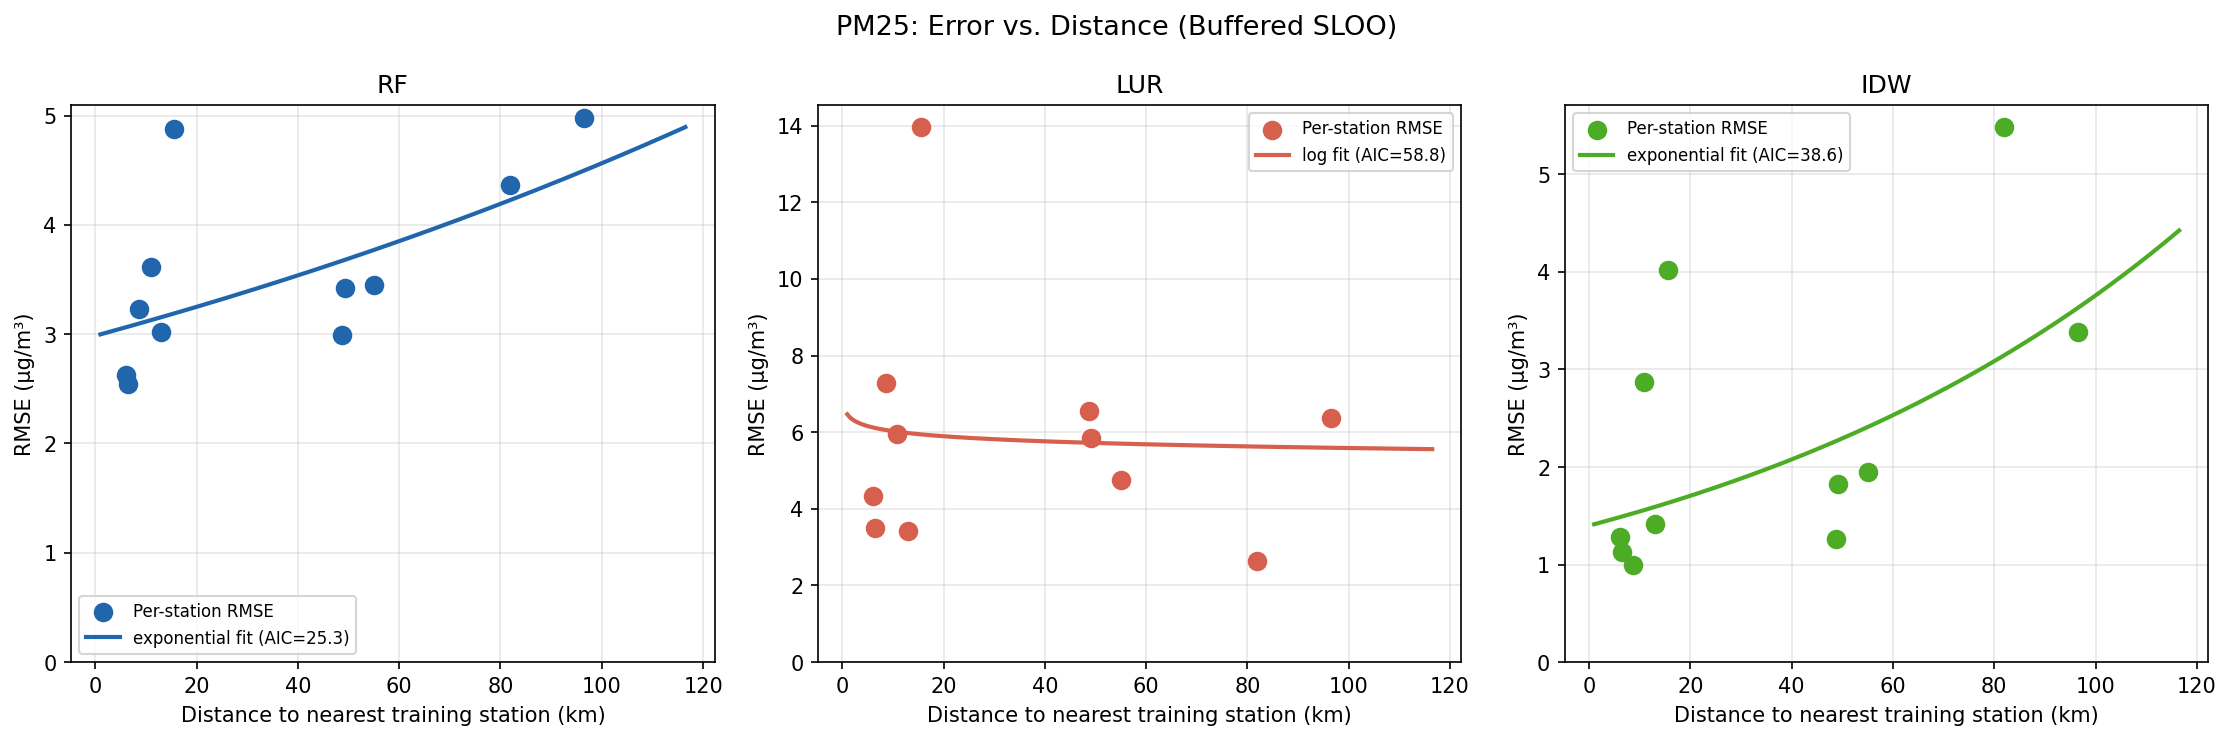
\includegraphics[width=\columnwidth]{fig_decay_pm25.png}
\caption{PM$_{2.5}$ error-distance decay under buffered SLOO for Random Forest,
LUR, and IDW. Points are per-station RMSE; the curve is the AIC-selected form.
The near-flat LUR fit reflects uniformly high error, not distance robustness.}
\label{fig:decay-pm25}
\end{figure}

\begin{figure}[t]
\centering
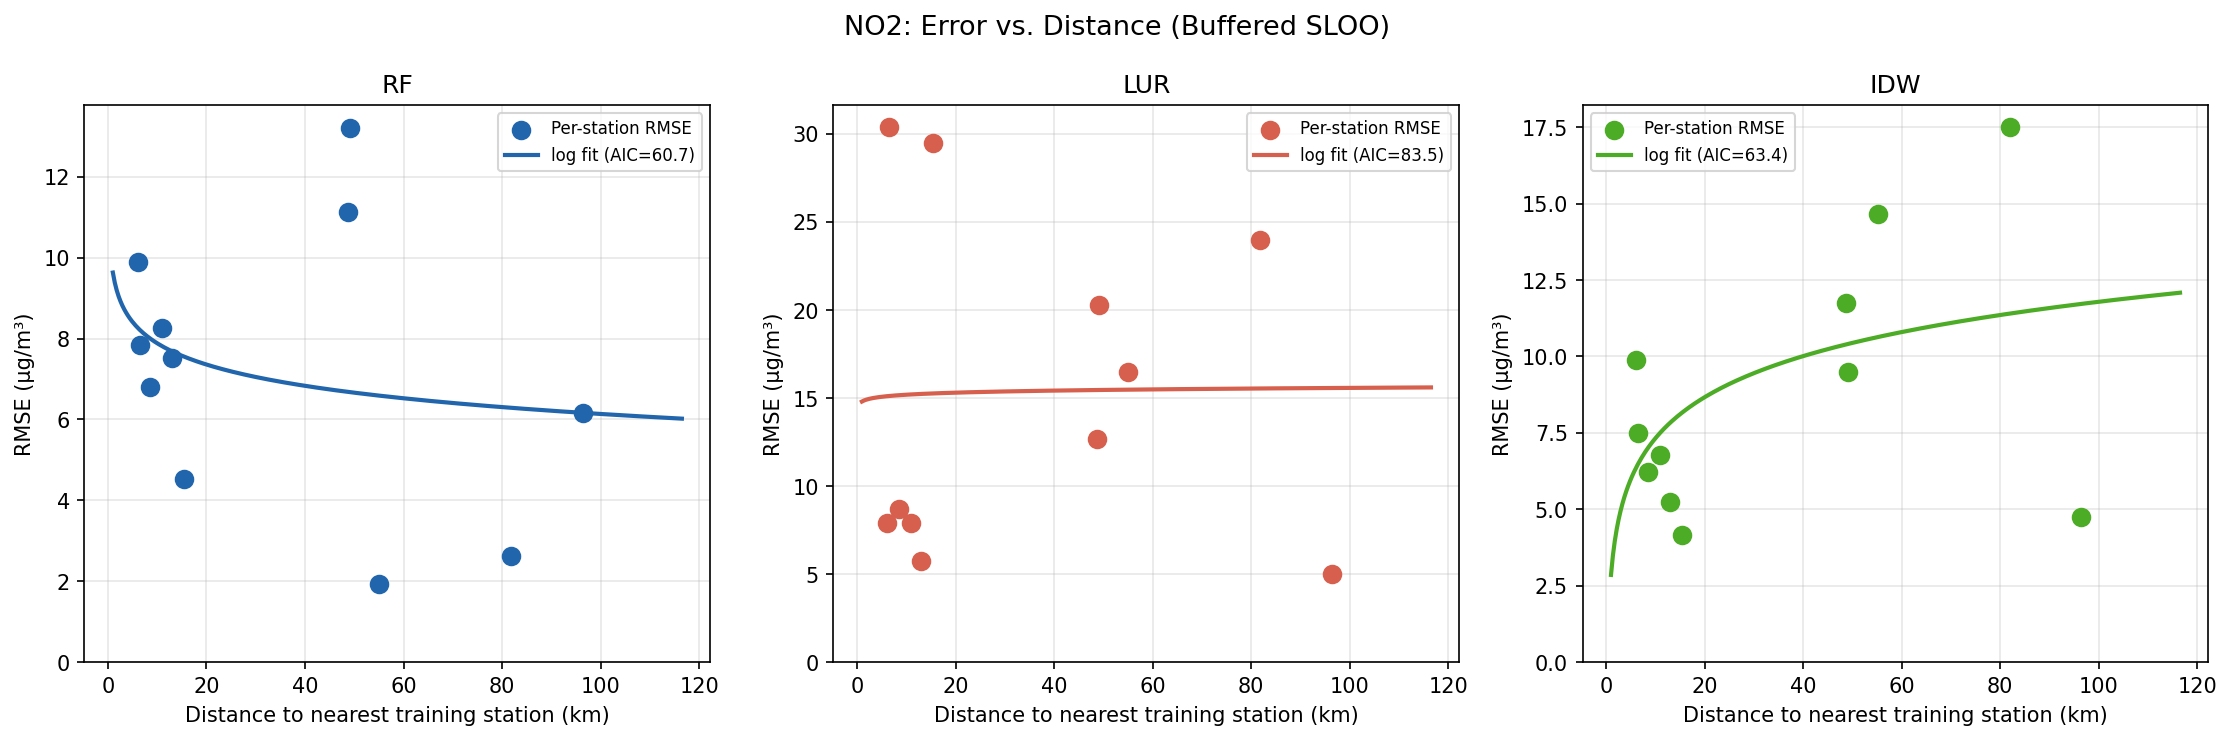
\includegraphics[width=\columnwidth]{fig_decay_no2.png}
\caption{NO$_2$ error-distance decay under buffered SLOO for Random Forest,
LUR, and IDW. Points are per-station RMSE; the curve is the AIC-selected form.
The near-flat LUR fit reflects uniformly high error, not distance robustness.}
\label{fig:decay-no2}
\end{figure}

\subsection{Sensor Placement (RQ3)}
\label{sec:results-rq3}

Under the 64~km PM$_{2.5}$ threshold, the 11 existing validation stations
cover 10.9~percent of Swedish land area and 38.8~percent of urban area. The
greedy algorithm places 20 sensors, distributed across G\"otaland (ranks
1--5), Svealand (ranks 6--11), and Norrland (ranks 12--20); each placement
adds the full 12{,}900~km$^{2}$ theoretical footprint, indicating no overlap
within the 20-sensor horizon. Coverage rises to 67.2~percent of land area and
71.4~percent of urban area, and population-weighted PM$_{2.5}$ coverage rises
from 45.0 to 77.1~percent. Four of the seven administrative regions currently
without a concurrent-passing station are served: J\"onk\"oping, \"Orebro,
Dalarna, and Norrbotten.

Evaluated against the 6~km NO$_2$ threshold, the same 20 sensors raise NO$_2$
land coverage only from 0.2 to 0.6~percent and leave urban coverage unchanged
at 6.1~percent. Table~\ref{tab:integrated} traces the full chain from
estimation accuracy through the distance threshold to the placement outcome.
The pollutant-specific spatial autocorrelation range measured for RQ1 sets the
threshold in RQ2, which sets the sensor budget required for national coverage
in RQ3, so a placement sized for PM$_{2.5}$ is by construction inadequate for
NO$_2$ at comparable cost.

\begin{table}[!ht]
\caption{Integrated results across the three research questions. Mean RMSE in
$\mu$g\,m$^{-3}$; coverage as land area / urban area, before $\rightarrow$
after the 20-sensor placement.}
\label{tab:integrated}
\centering
\footnotesize
\begin{tabular}{@{}lcc@{}}
\toprule
 & \textbf{PM$_{2.5}$} & \textbf{NO$_2$} \\
\midrule
RQ1: best estimator (mean RMSE) & IDW (2.33) & RF (7.27) \\
RQ2: reliable prediction distance & 64~km & 6~km \\
RQ3: land coverage & 10.9\% $\rightarrow$ 67.2\% & 0.2\% $\rightarrow$ 0.6\% \\
RQ3: urban coverage & 38.8\% $\rightarrow$ 71.4\% & 6.1\% $\rightarrow$ 6.1\% \\
\bottomrule
\end{tabular}
\end{table}

\begin{figure}[t]
\centering
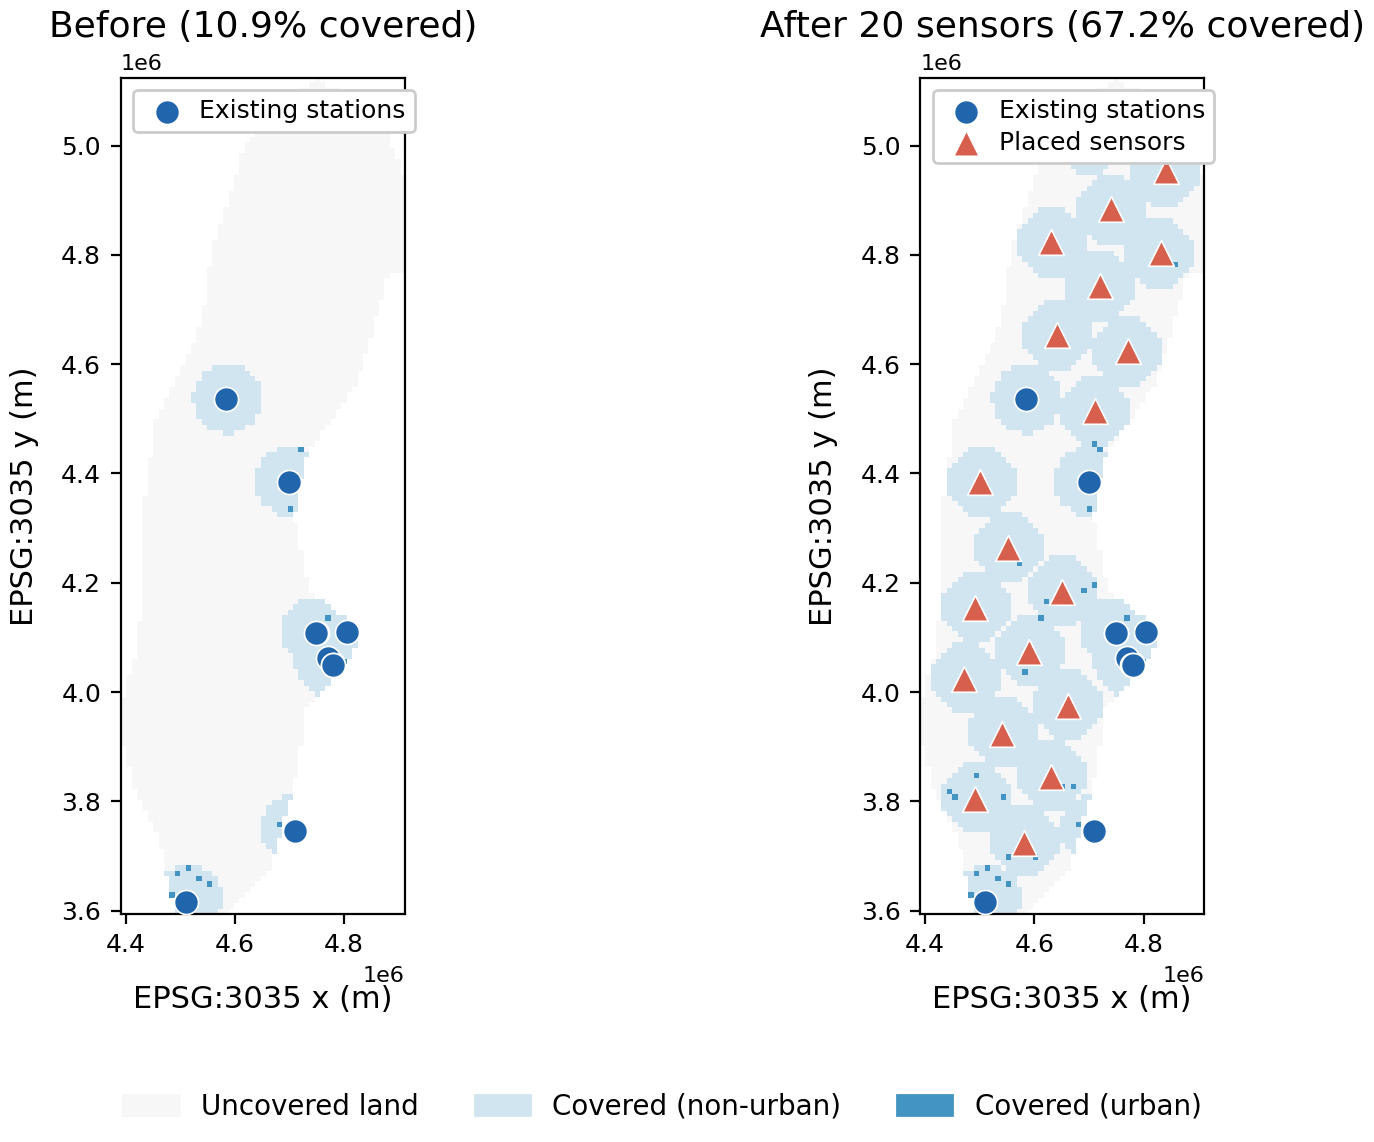
\includegraphics[width=\columnwidth]{fig_coverage_before_after_ieee.png}
\caption{PM$_{2.5}$ national coverage before (left) and after (right) 20
greedy placements, at the 64~km reliable prediction threshold. Grey cells are
beyond threshold; blue cells are covered land, with darker blue for covered
urban fabric. Circles mark existing stations; triangles mark recommended
sensor locations. Grid resolution 10~km.}
\label{fig:coverage}
\end{figure}
\FloatBarrier

\section{Discussion}
\label{sec:discussion}

The central result is an asymmetry. PM$_{2.5}$ and NO$_2$ differ by roughly an
order of magnitude in reliable prediction distance (64~km against 6~km), a
direct consequence of their spatial gradient behaviour: PM$_{2.5}$ has a
regional, mixed-source character that permits estimation across large
distances, whereas NO$_2$ has sharp, traffic-confined gradients. That IDW
outperforms Random Forest for PM$_{2.5}$ diverges from the general expectation
that feature-based learning beats deterministic interpolation
\cite{chen_pm25_interpolation_2021}, and is attributable to the sparse,
dispersed configuration of the Swedish network: when the autocorrelation range
is long relative to inter-station spacing, land-use, topographic, and
meteorological covariates add little. Both Random Forest and IDW exceed the LUR
benchmark for both pollutants, consistent with the broader machine learning
literature \cite{agbehadji_ml_aq_review_2024}, though a direct comparison with
the ESCAPE R$^2$ benchmarks is not straightforward, as those are derived from
annual means across 20 to 40 sites per area rather than daily series under
buffered SLOO. The constant marginal coverage gain across all 20 placements
indicates that the coverage landscape is not yet multimodal at this deployment
scale, the condition under which a population-based metaheuristic would be
expected to outperform greedy search \cite{gupta_pso_placement_2023}.

For municipal planning, the asymmetry means a single IoT deployment cannot be
sized for both pollutants from one threshold: the 20 PM$_{2.5}$-sited sensors
left NO$_2$ urban coverage unchanged. The two thresholds should be treated as
separate planning constraints, and the four served regions (J\"onk\"oping,
\"Orebro, Dalarna, and Norrbotten) as concrete near-term priorities.

Several limitations bound these findings. Only 11 stations pass the
completeness filter concurrently, well below ESCAPE-scale study areas, which
constrains the statistical power of the validation and the granularity of the
decay curves. The 5~km SLOO buffer is set by network clustering rather than
the variogram range, so reported errors are a lower bound. Euclidean distance
is used throughout, though road-network distance would be more appropriate for
NO$_2$. The NO$_2$ decay fit is confounded by having only two rural stations
in the sample. The 10~km placement grid is coarser than the 6~km NO$_2$
threshold, so it cannot resolve NO$_2$ coverage geometry. Finally, the
reported coverage percentages are contingent on the 50~percent criterion: the
same sensitivity sweep moves post-placement PM$_{2.5}$ land coverage across a
2.9 to 94.7~percent range. What is robust across that range is the
PM$_{2.5}$/NO$_2$ asymmetry itself.

\section{Conclusion}
\label{sec:conclusion}

This paper quantified how accurately PM$_{2.5}$ and NO$_2$ can be estimated at
unmonitored Swedish locations, how that accuracy decays with distance from the
nearest reference station, and how the resulting relationship guides
supplementary IoT sensor placement. Under buffered spatial leave-one-out
validation, Random Forest gave the lowest mean RMSE for NO$_2$
(7.27~$\mu$g\,m$^{-3}$) and inverse distance weighting for PM$_{2.5}$
(2.33~$\mu$g\,m$^{-3}$), with land-use regression least accurate for both.
Fitted decay curves yielded criterion-dependent reliable prediction distances
of approximately 64~km for PM$_{2.5}$ and 6~km for NO$_2$. Applying the
PM$_{2.5}$ threshold, a greedy sequential algorithm identified 20 candidate
sensor locations that raise national PM$_{2.5}$ land coverage from 10.9 to
67.2~percent and serve four of seven currently unmonitored regions, while the
same placement leaves NO$_2$ coverage essentially unchanged. The contribution
is a reproducible artefact linking a validated estimation model, a quantified
accuracy-distance relationship, and a transparent placement algorithm; it is a
data-driven starting point for planning, not an operational deployment plan or
a regulatory compliance assessment. Future work includes road-network distance
metrics for NO$_2$, denser validation via pooled Nordic reference networks,
and multi-objective placement on a finer grid.

\section*{Acknowledgment}

The author thanks Fisseha Mekuria for supervision and feedback throughout this
work. The study relies on open data from the Swedish Meteorological and
Hydrological Institute (air quality and meteorological observations), the
European Environment Agency and the Copernicus Land Monitoring Service (CORINE
Land Cover and EU-DEM), and Eurostat and the Joint Research Centre (the
GEOSTAT population grid).

\bibliographystyle{ieeetr}
\bibliography{IEEE-conference}

\end{document}
